\begin{center}{\Large \textbf{ Jahres\"uberblick der Saison 2018\footnote{f\"ur Winter 2017/18  Skitouren}}} 
\addcontentsline{toc}{section}{Jahres\"uberblick}

~

\begin{tabular}{lrr}
Skitouren & 2 & 120 \si{h\meter}\\
Radtouren& 0 & 0 \si{\kilo\meter}\\
Wanderungen& 1 & 650 \si{h\meter}\\
Klettern& 0&\\\hline
Total& 3 &
\end{tabular}\end{center}\newpage 
\begin{minipage}{\textwidth}\tour{Test}{2018-06-08}{10:00:00}{Skitour}[100 hm \&~10 km][01:00:00][02:00:00][Hier Begleitung eingeben...Test1]\label{2018-06-08-Test}Hier Beschreibung eingeben... Test


 Hier Kommentar eingeben...Test2
\end{minipage}\vspace{2em} ~\newline 
\begin{minipage}{\textwidth}\tour{Hot Springs}{2018-06-10}{10:18:00}{Wandern}[650 hm \&~20 km][05:00:00][05:55:00][Mihnea]\label{2018-06-10-Hot Springs}Test














 Test












\end{minipage}\newline\begin{tikzpicture} \pgfplotsset{ seconds to timeformat={x}{\hour:\minute}, }	\begin{axis}[xlabel=Hot Springs, xtick distance=2134.3, width=\linewidth, height=4cm, axis lines=left, no markers, grid=major, legend pos=south east]		\addplot [black] table {./tracks/src/2018-06-10_Hot Springs.csv};	\end{axis}	\end{tikzpicture}\begin{figure}\centering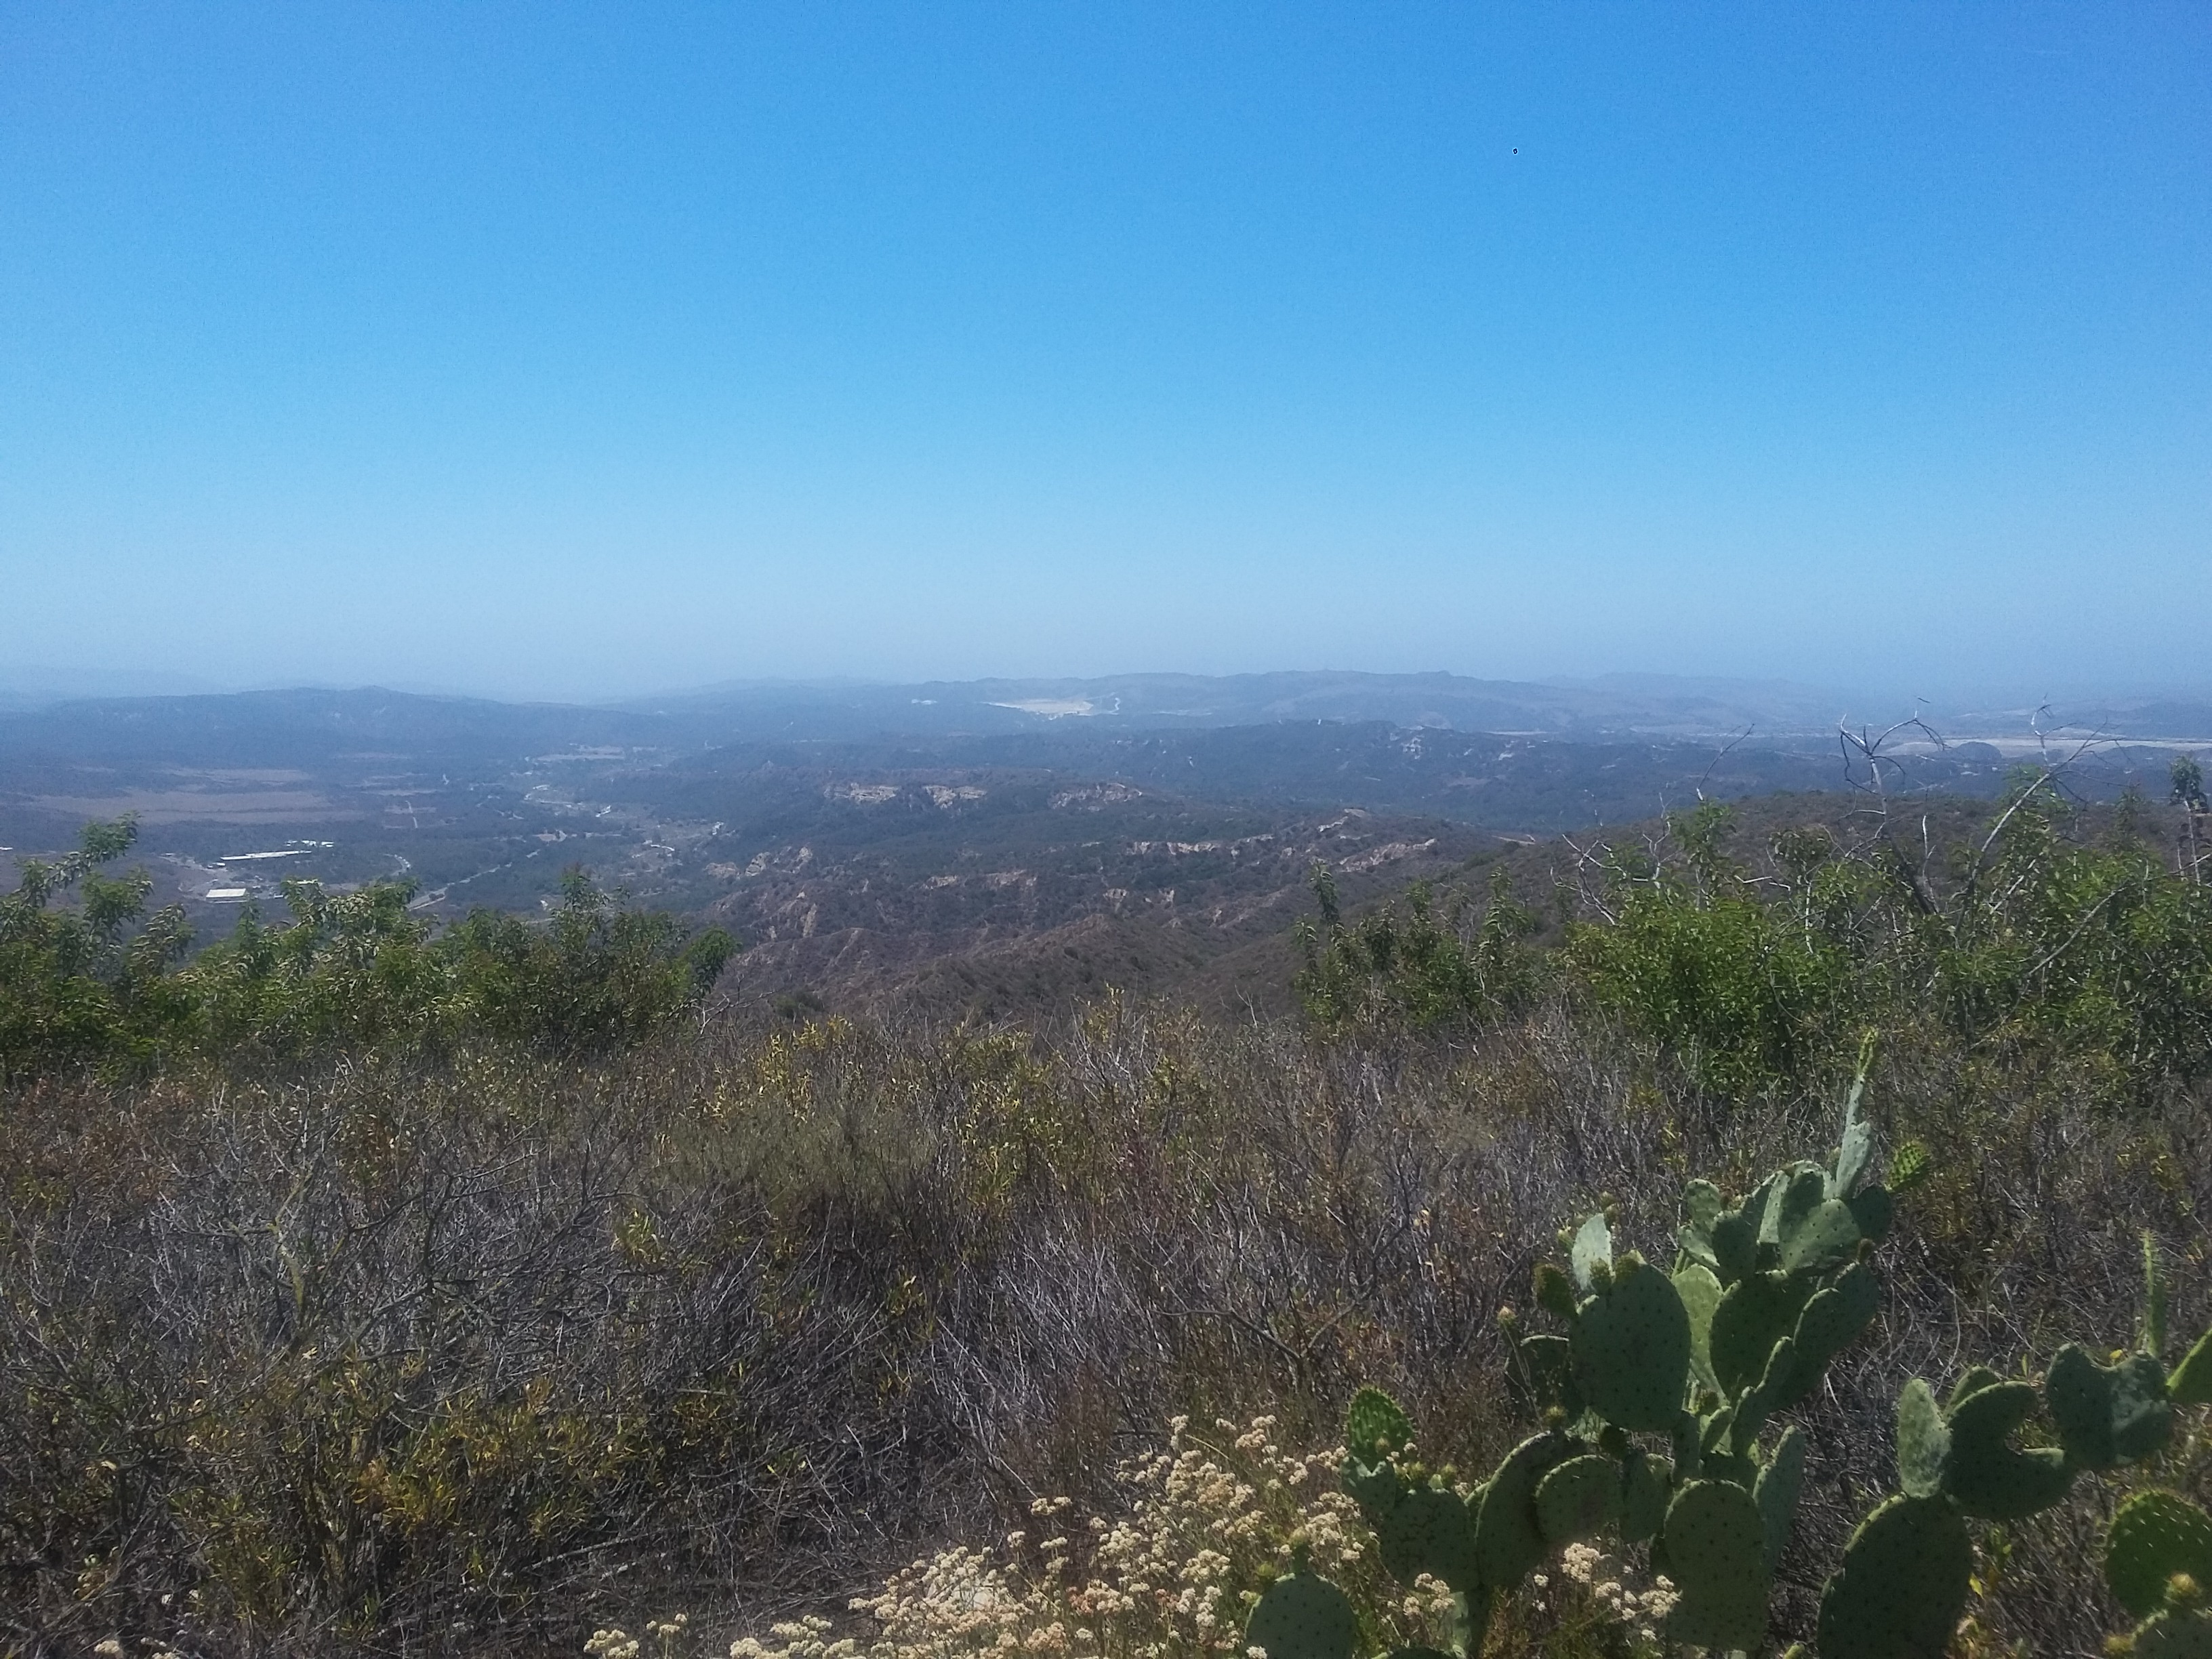
\includegraphics[angle=0,origin=c,height=0.25\textheight]{./Bilder/2018-06-10_Hot Springs/20180610_120436.jpg}\caption*{./2018-06-10\_Hot Springs/20180610\_120436.jpg}\end{figure}\begin{figure}\centering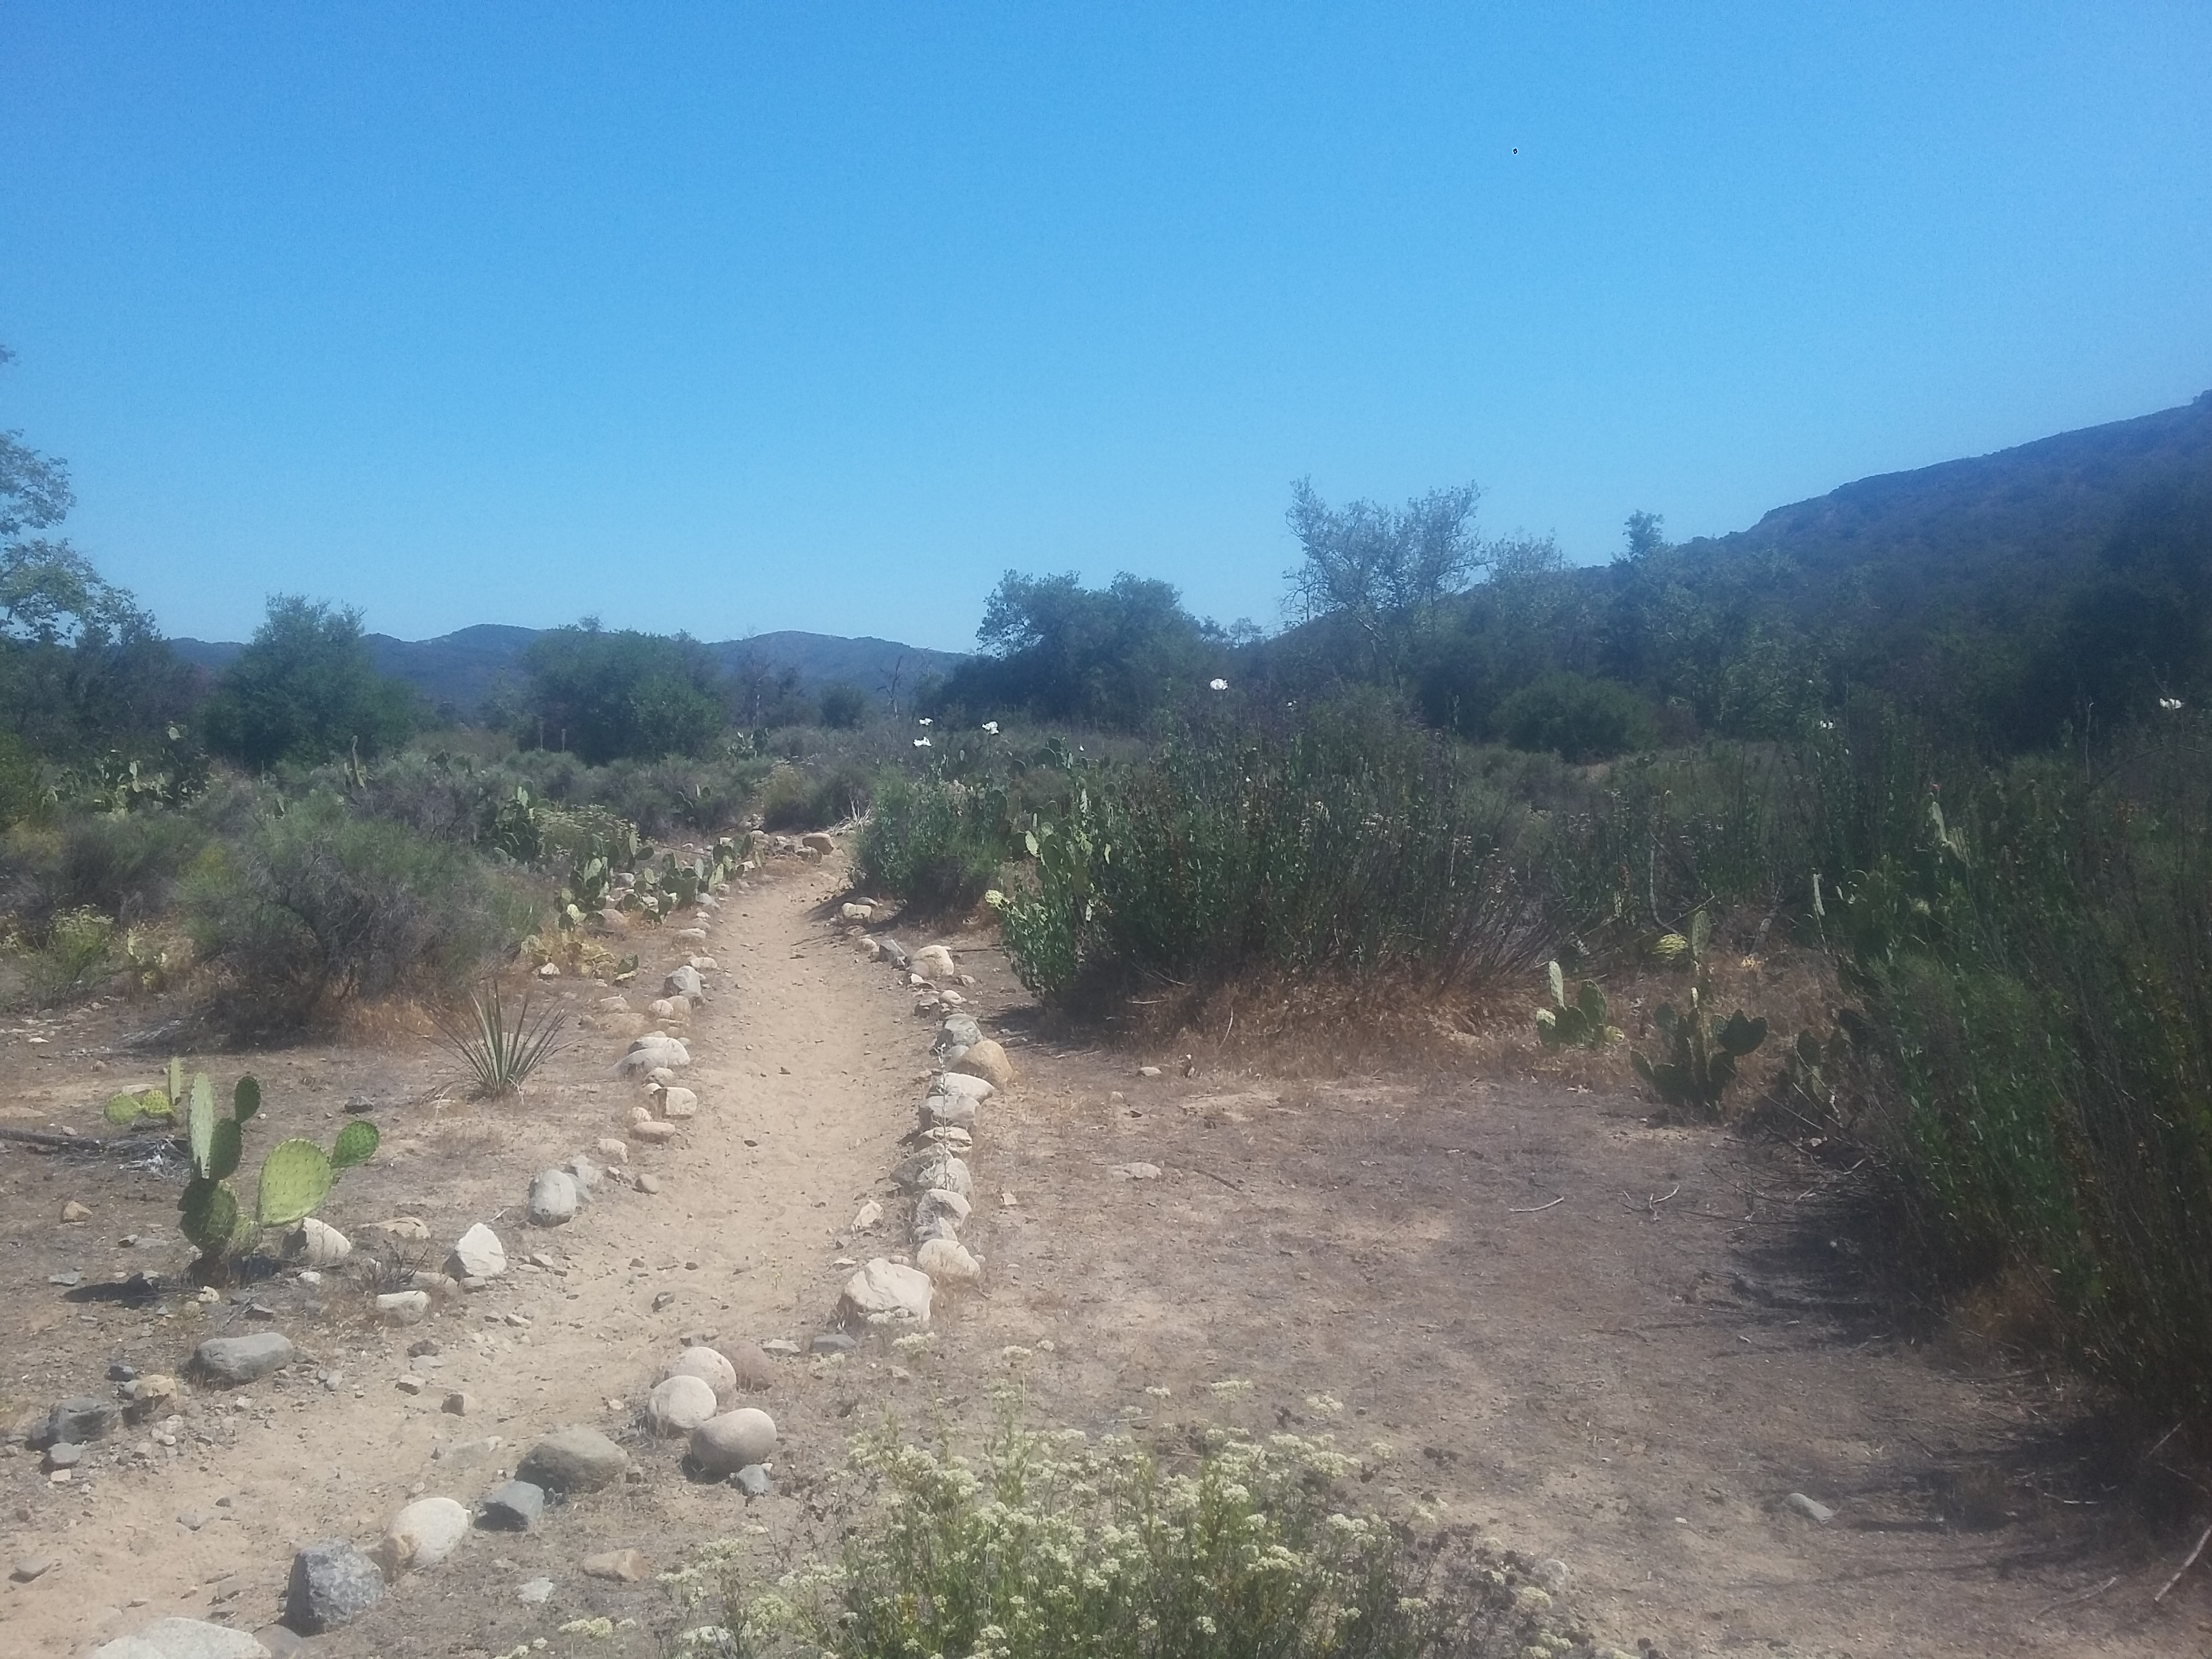
\includegraphics[angle=0,origin=c,height=0.25\textheight]{./Bilder/2018-06-10_Hot Springs/20180610_150223.jpg}\caption*{./2018-06-10\_Hot Springs/20180610\_150223.jpg}\end{figure}\vspace{2em} ~\newline 
\begin{minipage}{\textwidth}\tour{Test  1}{2018-06-24}{13:00:00}{Skitour}[20 hm \&~20 km][14:00:00][15:00:00][iHu1]\label{2018-06-24-Test  1}Hui1





 uiH1



\end{minipage}\begin{figure}\centering
\includegraphics[angle=0,origin=c,height=0.25\textheight]{./Bilder/2018-06-24_Test  1/SAVE.png}\caption*{./2018-06-24\_Test  1/SAVE.png}\end{figure}\begin{figure}\centering
\includegraphics[angle=0,origin=c,height=0.25\textheight]{./Bilder/2018-06-24_Test  1/Calendar.jpg}\caption*{./2018-06-24\_Test  1/Calendar.jpg}\end{figure}\vspace{2em} ~\newline 
